% Merkle batch commitment, two-layer label and the on-chain consume check.
\documentclass[tikz,border=2pt]{standalone}
\usepackage{newtxtext,newtxmath}
\usetikzlibrary{arrows.meta,positioning,patterns}
\newcommand{\qr}[2]{% #1 = centre, #2 = side (mm)
  \begin{scope}[shift={#1}]
    \fill[white] (-#2/2,-#2/2) rectangle (#2/2,#2/2);
    \foreach \x/\y in {0/0, 0.6/0.2, 0.2/0.6, 0.8/0.7, 0.45/0.45, 0.7/0.35, 0.3/0.15, 0.55/0.8}
      \fill (-#2/2+0.30*#2+\x*0.4*#2, -#2/2+0.30*#2+\y*0.4*#2) rectangle ++(0.09*#2,0.09*#2);
    \foreach \cx/\cy in {0/1, 1/1, 0/0} {
      \draw[line width=0.5pt] (-#2/2+\cx*0.72*#2+0.02*#2, -#2/2+\cy*0.72*#2+0.02*#2) rectangle ++(0.24*#2,0.24*#2);
      \fill (-#2/2+\cx*0.72*#2+0.08*#2, -#2/2+\cy*0.72*#2+0.08*#2) rectangle ++(0.12*#2,0.12*#2);
    }
  \end{scope}}
\begin{document}
\footnotesize
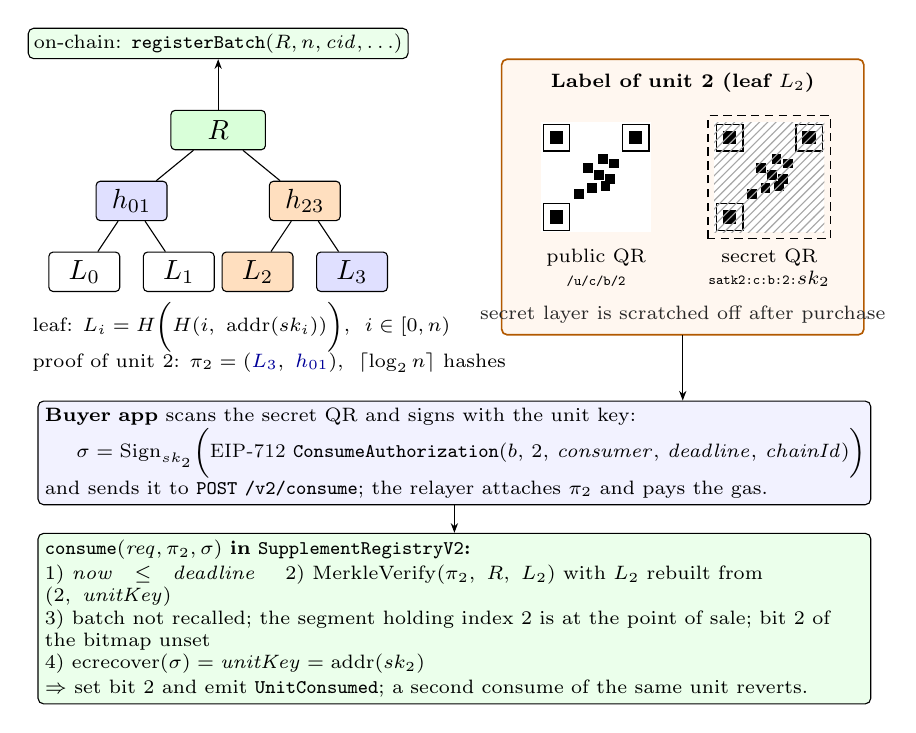
\begin{tikzpicture}[
  x=1mm, y=1mm,
  >={Stealth[length=3.5pt]},
  hash/.style={draw, rounded corners=1.5pt, minimum width=9mm, minimum height=5mm, inner sep=1pt, fill=white},
  path/.style={hash, fill=orange!25},
  sib/.style={hash, fill=blue!12},
  lbl/.style={font=\scriptsize, inner sep=1pt},
  box/.style={draw, rounded corners=2pt, align=left, font=\scriptsize, inner sep=2.5pt, text width=104mm},
]
  % ---------------- Merkle tree over the lot
  \node[draw, rounded corners=2pt, fill=green!8, lbl, inner sep=2pt] (chain) at (22,11)
    {on-chain: \texttt{registerBatch}$(R, n, \mathit{cid}, \dots)$};
  \node[hash, fill=green!15, minimum width=12mm] (root) at (22,0) {$R$};
  \node[sib] (h01) at (11,-9) {$h_{01}$};
  \node[path] (h23) at (33,-9) {$h_{23}$};
  \node[hash] (l0) at (5,-18) {$L_0$};
  \node[hash] (l1) at (17,-18) {$L_1$};
  \node[path] (l2) at (27,-18) {$L_2$};
  \node[sib] (l3) at (39,-18) {$L_3$};
  \foreach \a/\b in {root/h01, root/h23, h01/l0, h01/l1, h23/l2, h23/l3} \draw (\a) -- (\b);
  \draw[->] (root) -- (chain);
  \node[lbl, anchor=west] at (-2,-25) {leaf: $L_i=H\big(H(i,\ \mathrm{addr}(sk_i))\big)$, \ $i\in[0,n)$};
  \node[lbl, anchor=west] at (-2,-29.5) {proof of unit 2: $\pi_2=(\textcolor{blue!60!black}{L_3},\ \textcolor{blue!60!black}{h_{01}})$, \ $\lceil\log_2 n\rceil$ hashes};

  % ---------------- two-layer label of unit 2
  \begin{scope}[shift={(81,-8)}]
    \draw[rounded corners=2pt, fill=orange!6, draw=orange!70!black, line width=0.6pt] (-23,-18) rectangle (23,17);
    \node[lbl, font=\scriptsize\bfseries] at (0,14) {Label of unit 2 (leaf $L_2$)};
    \qr{(-11,2)}{14}
    \node[lbl, align=center] at (-11,-9.5) {public QR\\\texttt{\tiny /u/c/b/2}};
    \qr{(11,2)}{14}
    \fill[pattern=north east lines, pattern color=gray!70] (4,-5) rectangle (18,9);
    \draw[densely dashed] (3.2,-5.8) rectangle (18.8,9.8);
    \node[lbl, align=center] at (11,-9.5) {secret QR\\\texttt{\tiny satk2:c:b:2:}$sk_2$};
    \node[lbl, text=gray!30!black] at (0,-15.5) {secret layer is scratched off after purchase};
  \end{scope}

  % ---------------- consume
  \node[box, fill=blue!5] (sig) at (52,-41)
    {\textbf{Buyer app} scans the secret QR and signs with the unit key:\\
     \hspace*{4mm}$\sigma=\mathrm{Sign}_{sk_2}\big(\textsc{EIP-712}\ \texttt{ConsumeAuthorization}(b,\,2,\,\mathit{consumer},\,\mathit{deadline},\,\mathit{chainId})\big)$\\
     and sends it to \texttt{POST /v2/consume}; the relayer attaches $\pi_2$ and pays the gas.};
  \node[box, fill=green!8, below=3.5mm of sig] (check)
    {\textbf{\texttt{consume}$(\mathit{req},\pi_2,\sigma)$ in \texttt{SupplementRegistryV2}:}\\[1pt]
     1) $\mathit{now}\le\mathit{deadline}$ \quad 2) $\mathrm{MerkleVerify}(\pi_2,\ R,\ L_2)$ with $L_2$ rebuilt from $(2,\ \mathit{unitKey})$\\
     3) batch not recalled; the segment holding index 2 is at the point of sale; bit 2 of the bitmap unset\\
     4) $\mathrm{ecrecover}(\sigma)=\mathit{unitKey}=\mathrm{addr}(sk_2)$\\[1pt]
     $\Rightarrow$ set bit 2 and emit \texttt{UnitConsumed}; a second consume of the same unit reverts.};
  \draw[->] (81,-26) -- (81,0 |- sig.north);
  \draw[->] (sig) -- (check);
\end{tikzpicture}
\end{document}
